\chapter{Results}
\section{Neutral Simulations}
To demonstrate how altering some parameters changes the dynamics of our model, we present a collection of simulated allele frequency trajectories in a one-deme, neutral Wright-Fisher model ($\mu = s = m = 0$). We vary the population size $N$ and the initial allele frequency $f_0$ and observe changes due to genetic drift. Recall the following properties:

\begin{equation}
    \tag{\ref{eq:ex_drift} revisited}
    E[f_t] = f_0
\end{equation}

\begin{equation}
    \tag{\ref{eq:var_lim_drift} revisited}
    \lim_{N \to \infty} Var[f_{t+1}|f_t] = 0
\end{equation}


Figure (\ref{fig:neutral_wf}) neatly demonstrates these properties while also illustrating the time dynamics of the neutral Wright-Fisher model. We validate our analytical predictions of $E[f] = f_0$ for the neutral Wright-Fisher model. Figure \ref{fig:mean_wf} shows that the average frequency computed from simulated data matches the set initial frequency. As $N \to \infty$, the deviation from this prediction becomes $0$, but at small population sizes, changes due to drift introduce errors in our predictions. 


\begin{figure}[H]
    \centering
    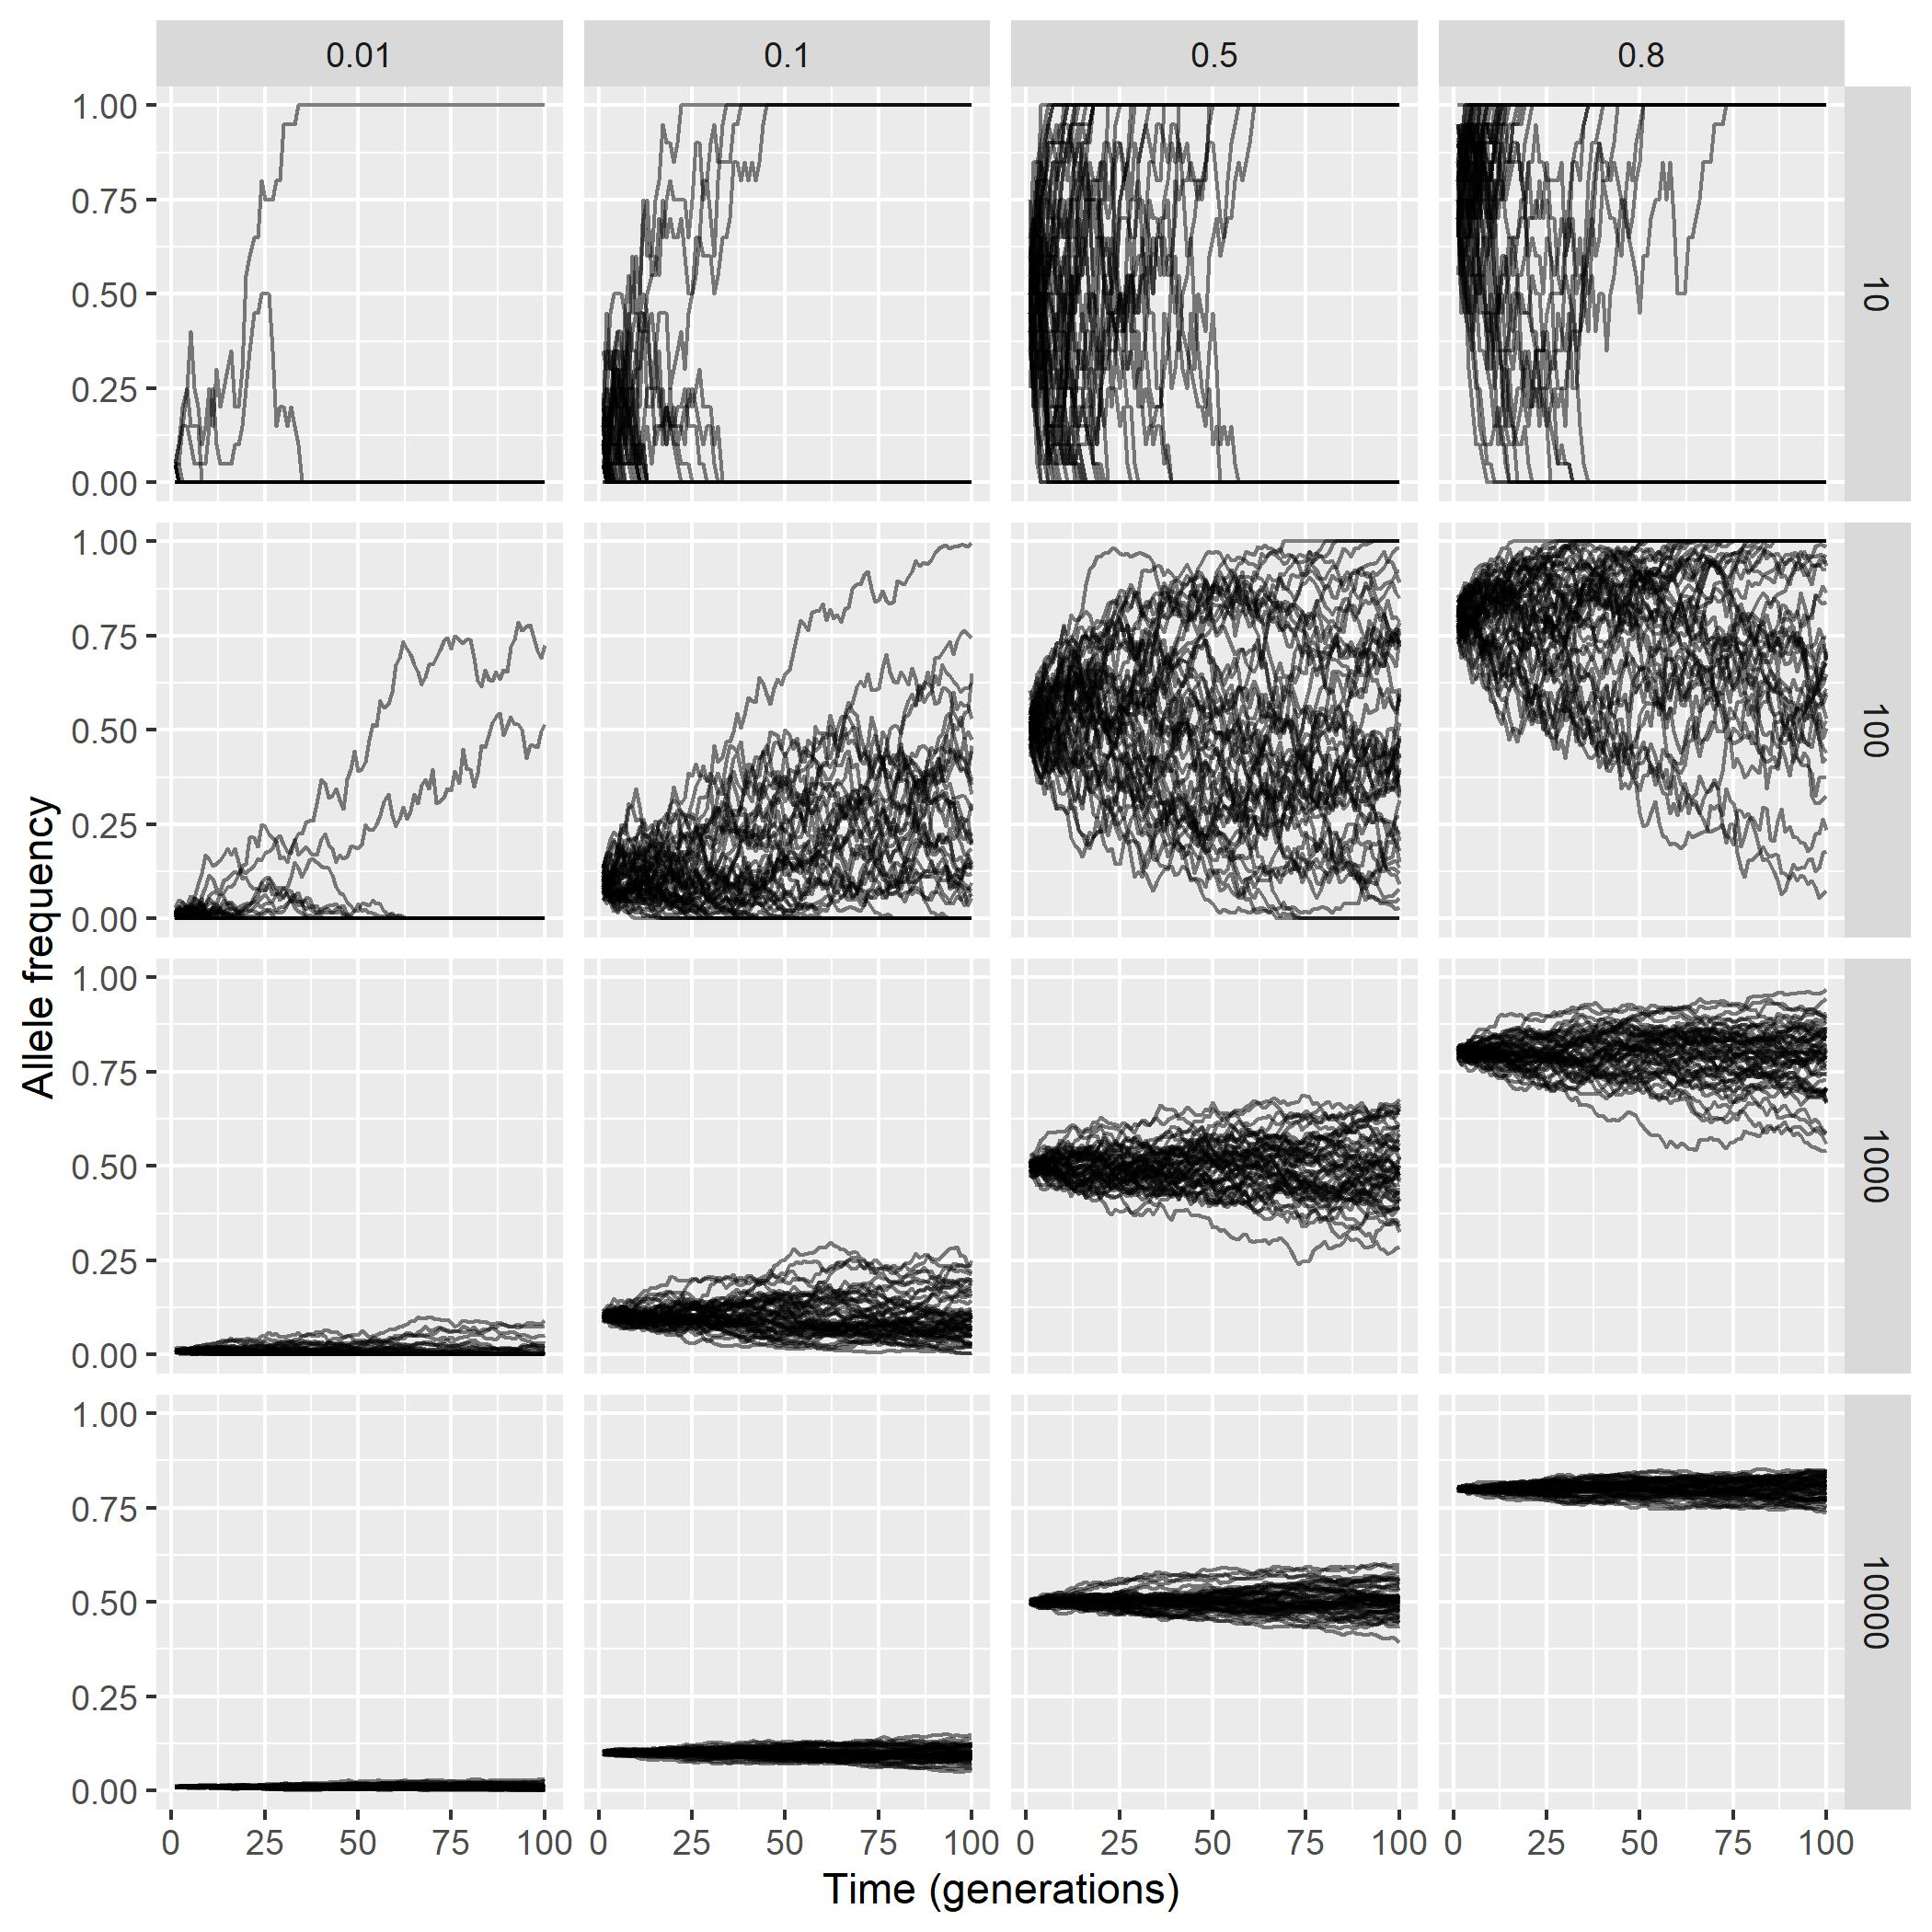
\includegraphics[scale=0.8]{img/neutral_wf.jpg}
    \caption{This figure shows several simulated trajectories for varying initial allele frequency $f_0$ and population size $N$ in a one deme, neutral Wright-Fisher model. Each row shows simulations run with a common $N$ and each column shows a common $f_0$. Figure formatting is inspired by Novembre lab member Joe Marcus' \textit{Introduction to the Wright-Fisher model}.\cite{marcus_introduction_2016}}
    \label{fig:neutral_wf}
\end{figure}


\begin{figure}[H]
    \centering
    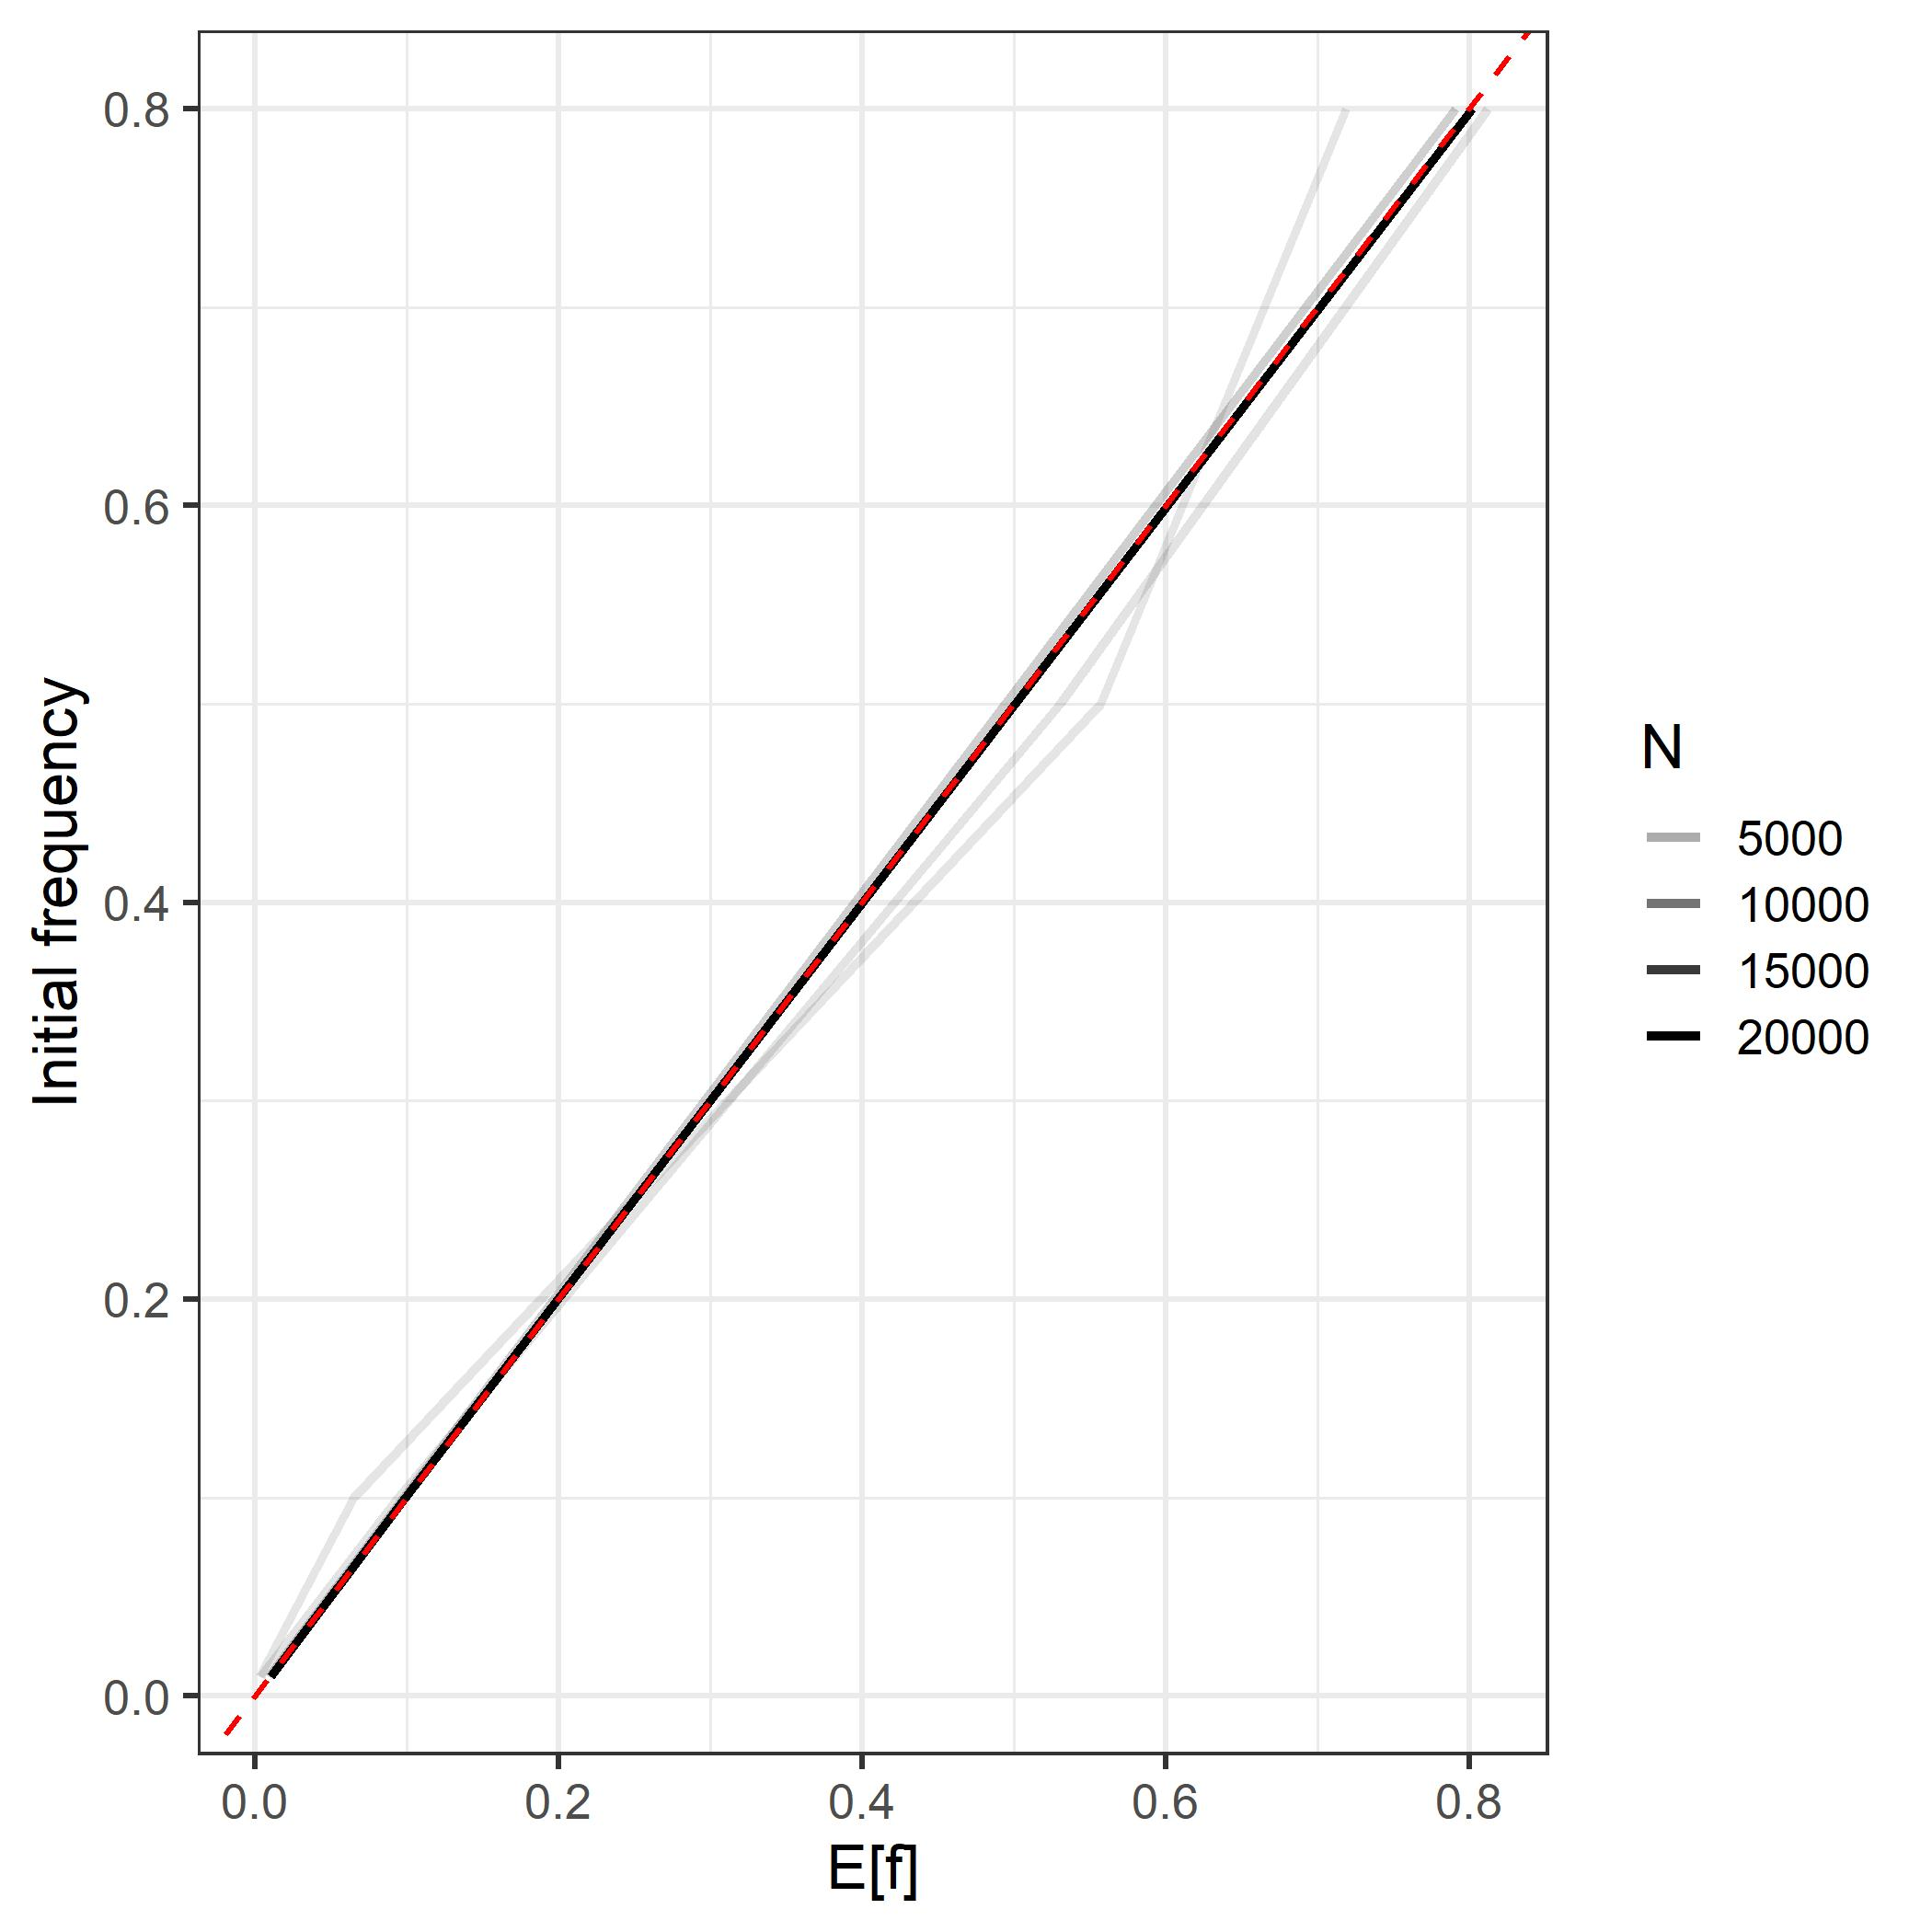
\includegraphics[scale=0.5]{img/mean_f.jpg}
    \caption{This figure confirms the neutral Wright-Fisher model average frequency. As predicted, $E[f] = f_0$. Simulations run at varying population sizes validate this prediction. The dashed, red line has y-intercept $0$ and slope $1$.}
    \label{fig:mean_wf}
\end{figure}


\section{Important Quantities from Our Model}
As shown in the previous chapter, our model describes the change in allele frequencies over time and space. Evolutionary forces act to shape the distribution of alleles across our simulated geographic habitat. There are two immediate questions that we will utilize our model to answer:

\begin{enumerate}
    \item How much of the allele do we expect to observe?
    \item Where can we expect to find the allele?
\end{enumerate}


For a more intuitive understanding of what each of these questions represent, let us examine the raw simulation output from our model. We simulate a single genetic locus and record the frequency of the minor, or \textit{focal} allele $f(a)$ after thousands of simulated generations. Allele frequencies vary across geographic position, but tend to be higher in some neighboring demes. This represents the localization of rare alleles observed in natural populations. \cite{1k_genomes} \cite{geerlings_geographic_2018} \cite{marcus_visualizing_2017} 


\begin{figure}[H]
    \centering
    \textbf{Allele frequency heatmap in 2D simulation} \par \medskip
    \hspace*{+1.5cm}  
    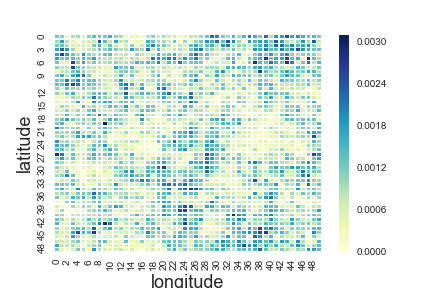
\includegraphics[scale=1]{img/heatmap.png}
    \caption{The geographic distribution of allele frequencies in a single simulation with a single set of evolutionary parameters ($\mu = 10^{-5},s = 10^{-2},m=10^{-1},N=10^{4}$). We allow for thousands of generations of time to pass to allow our simulation to approach equilibrium. Alleles exist in clusters throughout the spatial environment.}
    \label{fig:geog_sim}
\end{figure}


We observe that demes with the highest focal allele frequencies tend to exist in clusters (Figure: \ref{fig:geog_sim}). The size of these clusters illustrate the geographic range of the allele. New alleles come into existence at one particular location. Some of these will reach higher frequencies in the population and some will spread farther beyond their initial position. The average frequency in these clusters tells us how much of the allele we can expect to observe, and the size of the clusters tells us where we can expect to observe it. It is clear that alleles that reach, on average, higher frequencies will be easier to observe. We will calculate the average allele frequency and the geographic range of an allele analytically and confirm our predictions with simulation data.


\subsection{The average allele frequency}
Recall that we simulate changes in allele frequency according to the equation:

\begin{equation}
    \tag{\ref{eq:model} revisited}
    X_r(t+1) | \hat{f}(t) \sim Binom(N,f_r(t+1))
\end{equation}

Where $f_r(t+1)$ is given by:

\begin{equation}
    \tag{\ref{eq:f_r,t} revisited}
    f_r(t+1) = \mu(1-2f_r)-sf_r (1-f_r) + m (f_{r-1}+f_{r+1}-2f_r)
\end{equation}

We want to solve this equation for the average, or expected, allele frequency at equilibrium $E_{r,t}[f_{t+1} | f_t] = E[f_t] = f_0 = 0$. We take the expectation over $t$ and $r$. Using the Law of Total Expectation, we can show:

\begin{equation}
    \begin{split}
        0 &= E[\mu(1-2f_r)-sf_r (1-f_r ) + m (f_{r-1}+f_{r+1}-2f_r)] \\ 
        & \text{Using equation \ref{eq:exp_ss}:} \\
        &= E[\mu(1-2f_r)-sf_r (1-f_r )] + 0   \\
        &= E[\mu(1-2f_r)] - E[sf_r (1-f_r)] \\
        &= \mu - 2\mu E[f] - sE[f] + sE[f^2] \\
        E[f](2\mu + s) &= \mu + sE[f^2] \\
        E[f] &= \frac{\mu + sE[f^2]}{2\mu + s} \\
        & \text{Using $sE[f^2] << \mu$ (rare allele assumption):} \\
        E[f] &\approx  \frac{\mu}{2\mu + s}  \\
        & \text{Using $2\mu << s$: (strong selection assumption):} \\
        \therefore E[f] &\approx \frac{\mu}{s} 
    \end{split}
\end{equation}


Thus, even with geographic population structure, our model accords with the well-known \textit{mutation-selection balance} result \cite{fisher_genetical_1930} in well-mixed populations. The average allele frequency can be approximated as the ratio of the mutation rate to the selection coefficient. As we increase the selection coefficient, selection removes the allele from the population at a faster rate. This implies that the allele will be rarer on average. note that this result is independent of population size and migration. We validate this relationship with simulations:

\begin{figure}[H]
    \centering
    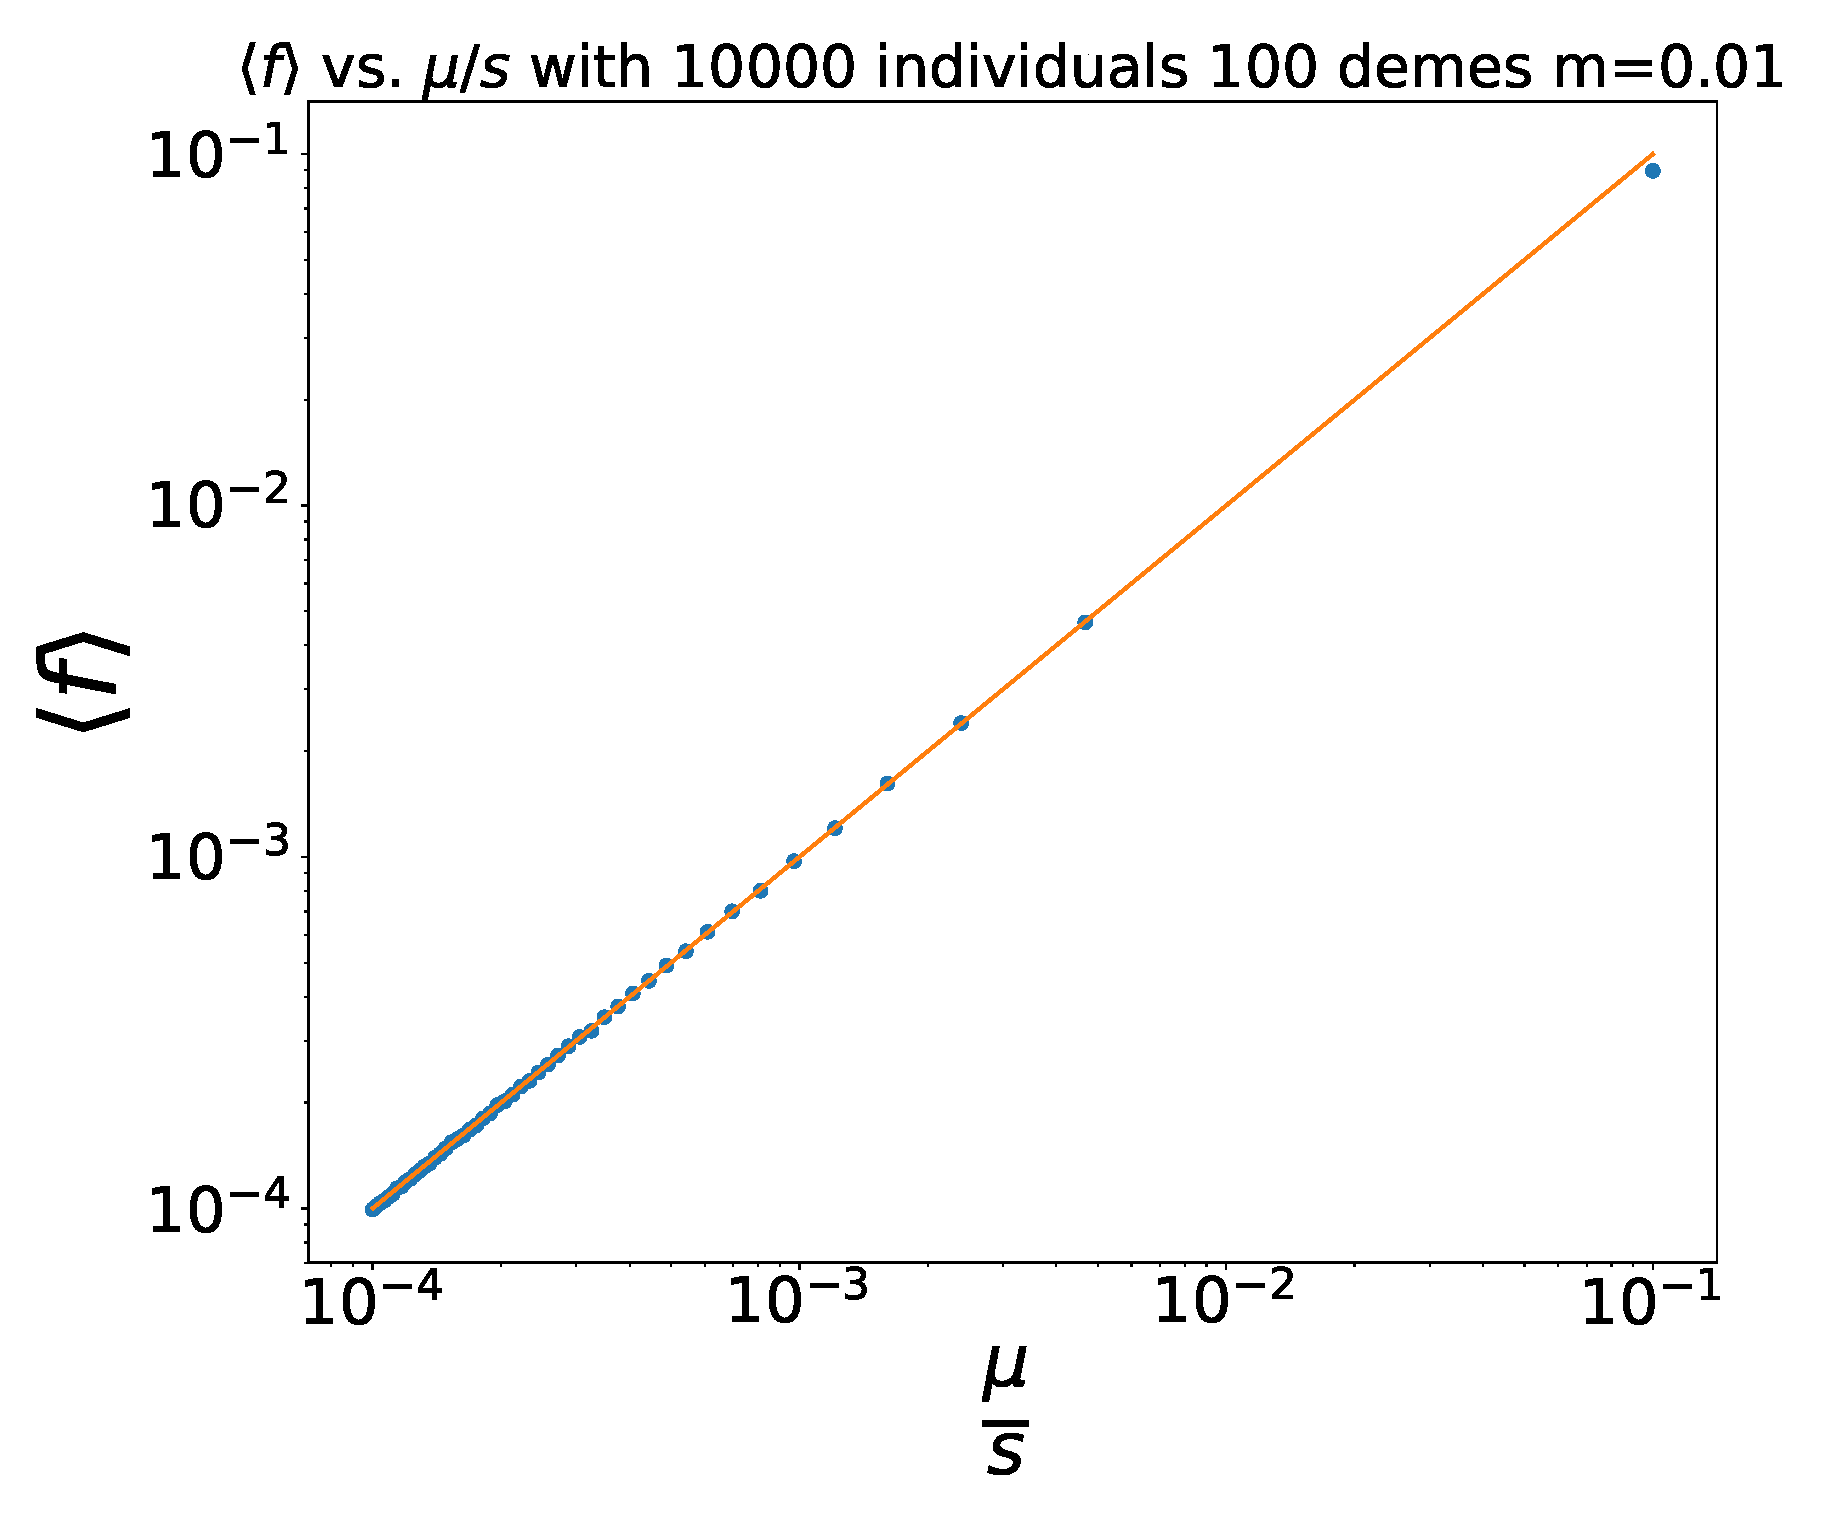
\includegraphics[scale=0.4]{img/fig1.eps}
    \caption{The average allele frequency $E[f] = \langle f \rangle$ is proportional to the ratio $\frac{\mu}{s}$. Each point shows the computed mean frequency value from a simulation run to equilibrium and the mutation-selection ratio used. The line shown has slope $1$ and intercept $0$. }
    \label{fig:avg_freq}
\end{figure}

$\frac{\mu}{s}$ tells us, on average, how much of the allele we expect to observe at any location. The mutation rate in mammalian genomes is approximately constant across genes (order $10^{-9}$ per base pair per year). \cite{kumar_mutation_2002} \cite{scally_mutation_2016} Therefore, the main force driving average allele frequencies is selection. This result validates our previous intuition that large-effect/largely deleterious alleles tend to be rare.

\newpage
\subsection{The geographic range of the allele}
In this section we examine the forces driving the geographic range of the allele. We expect rare alleles to be more geographically isolated, and we have just shown that selection determines allele rarity. Therefore, we are particularly interested in how changing rates of selection and migration influences the geographic patterns of allele frequencies. 


Let us examine the parameters $m$ and $s$ in relation to one another. Both parameters are of dimensions $[m] = [s] = [time^{-1}]$. Therefore, their reciprocals are of dimensions $[time]$. The value $\frac{1}{m}$ is essentially the time an allele takes to migrate between demes. Another way to interpret this is that \textit{increasing} $m$ \textit{decreases} the time an allele spends in the same deme. Likewise, the value $\frac{1}{s}$ is essentially the time before an allele is removed by selection, i.e. the \textit{lifespan} of the allele. We examine the three possible relationships:

\noindent\begin{tabularx}{\textwidth}{@{}XXX@{}}
  \begin{equation} 
           \frac{1}{s} < \frac{1}{m}
    \implies \frac{m}{s} < 1 
    \label{eq:ms_less_1}
  \end{equation} &
  \begin{equation}
           \frac{1}{s} = \frac{1}{m}
    \implies \frac{m}{s} = 1 
    \label{eq:ms_equal_1}
  \end{equation} &
  \begin{equation}
           \frac{1}{s} > \frac{1}{m}
    \implies \frac{m}{s} > 1 
    \label{eq:ms_greater_1}
  \end{equation}
\end{tabularx}

Inequality \ref{eq:ms_less_1} states that the lifespan of an allele is shorter than the time it takes the allele to move to another deme. In this scenario, we expect changes in the allele frequency at one deme to not strongly affect the allele frequency in nearby demes. Changes in allele frequencies in nearby demes should be mostly \textit{uncorrelated}. If \ref{eq:ms_equal_1} is true, then neither force has an advantage over the other and we expect to see some correlation of allele frequencies in nearby demes. Some alleles have time to migrate to nearby demes before they are removed by selection. The final case of inequality \ref{eq:ms_greater_1} predicts that alleles have lifespans longer than the time it takes them to migrate. Therefore, we expect to see strong correlation in allele frequencies of nearby demes. We simulate frequency trajectories in a two-deme model under each of the three possible $\frac{m}{s}$ relationships. $\frac{\mu}{s}$ is kept constant for each simulation, so only $m$ is increased.


\begin{figure}[H]
    \centering
    \hspace*{-2cm}
    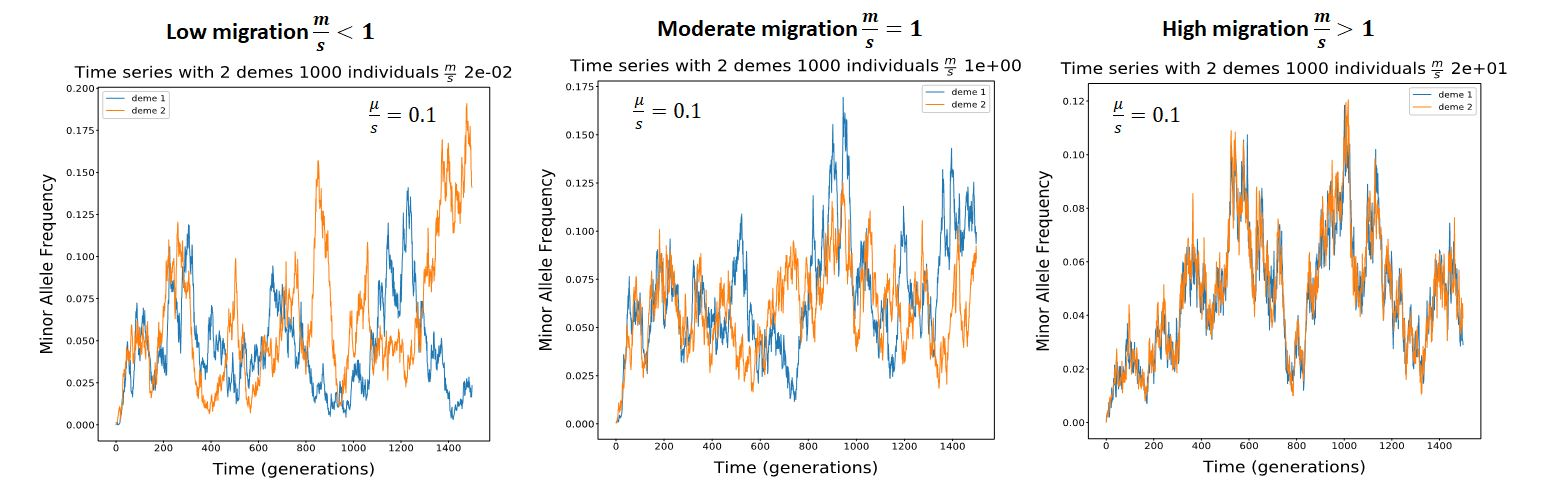
\includegraphics[scale=0.5]{img/low_high_migration.JPG}
    \caption{As the migration rate increases, we observe stronger coupling in the frequencies of two neighboring demes.}
    \label{fig:low_high_m}
\end{figure}


Let us explicitly quantify the change in allele frequency correlation for a one-dimensional spatial model. We denote the correlation between allele frequencies separated by a distance $d$ as:

\begin{equation}
    Corr[f_r,f_{r+d}] = E[f_r f_{r+d}] - E[f_r] E[f_{r+d}] = E[(f_r - E[f])(f_{r+d} - E[f])]
\end{equation}

We can take advantage of the \textit{translational invariance} in $r$ (symmetric boundaries of the Stepping Stone model) to approximate the correlation function solely in terms of $d$.

\begin{equation}
    Corr[d] \approx \frac{1}{L} \sum_{r=1}^L (Corr[f_r,f_{r+d}]) = Ce^{\frac{-d}{d_c}} \tag{Kimura and Weiss (1964) \cite{kimura_stepping_1964}}
\end{equation}

We see that correlation is expected to decay exponentially as a function of distance between pairs of demes $d$. Demes that are farther apart in the Stepping Stone model will have approximately independent changes in allele frequencies. Notice that the rate of decay in correlation is determined by a critical distance $d_c$. We define $d_c$ as the following:

\begin{equation}
    d_c = \sqrt{\frac{m}{s}}
\end{equation}


$d_c$ determines the rate at which correlation decays. Increasing $m$ increases $d_c$ which slows the rate of correlation decay because alleles can migrate more quickly to nearby demes, resulting in stronger coupling (figure \ref{fig:low_high_m}). Plotting correlation vs. $\frac{d}{d_c}$ normalizes the difference in decay rate between simulations. Each curve falls roughly along the same path. This implies that $d_c$ is the rate of allele spread over the simulated geographic environment. Rare alleles tend to be found within $d_c$ of their location.


\begin{figure}[H]
    \centering
    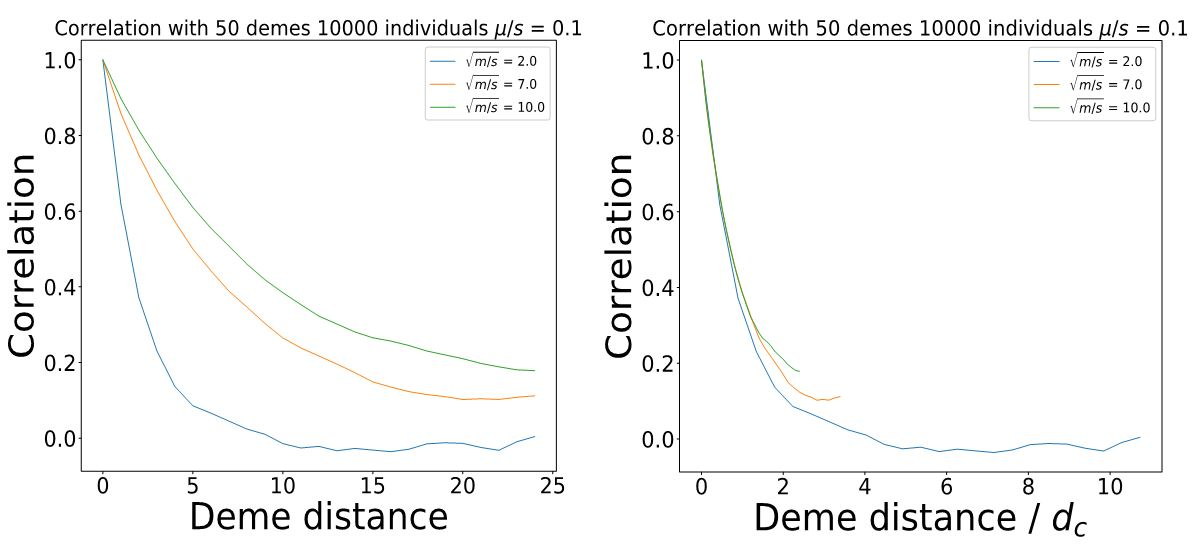
\includegraphics[scale=0.5]{img/correlation_curve.JPG}
    \caption{Correlation decays exponentially as a function of deme distance $d$. Each curve shows correlation calculated from a simulation run with different $m$ to change $d_c = \sqrt{\frac{m}{s}}$. Normalizing by $d_c$ results in each curve decaying at roughly the same rate.}
    \label{fig:correlation}
\end{figure}


In this section, we've identified two important quantities that influence allele detection:

\begin{enumerate}
    \item $\frac{\mu}{s}$ determines how much of the allele we expect to observe
    \item $\sqrt{\frac{m}{s}}$ determines the geographic range of the allele
\end{enumerate}



\newpage
\section{Computing the Expected Site Frequency Spectrum}
Here we present the effect of the GWAS sampling process on the expected distribution of allele frequencies, also known as the \textit{site frequency spectrum} (SFS). We ask the following question:

\begin{center}
    \textit{What is the probability of observing $j$ allele copies out of \\
    a sample of $n$ individuals in the population?}
\end{center}

The expected SFS summarizes these probabilities. Recall our methods of sampling from the simulated distribution of allele frequencies (equation \ref{eq:convolution}). We produce a matrix $\textbf{F}$ that contains allele frequencies for each deme sampled according to a Gaussian distribution of width $w$. To show the probability of observing $j$ allele copies out of $n$ individuals, we use $\bf{F}$. We can compute the expected SFS $\xi_{j,n}$ as a function of $j,n$ using the probability mass function of the binomial distribution:

\begin{equation}\label{eq:sfs}
    \xi_{j,n} = E[{n \choose j} F_w^j(1-F_w)^{n-j}]
\end{equation}


Note that we are discussing two separate "sampling" processes. The first being our approach to simulate the process by which GWAS designers select individuals for a cohort (contained in \textbf{F}), and the second being the process by which we summarize the observations of the GWAS sample (contained in the expected SFS). We compute the expected SFS for a range of sampling widths $w$ and demonstrate the decline in the probability of observing multiple copies of the minor allele in a sample of size $n$ (figure \ref{fig:sfs}). Broader sampling width $w$ increases the rate at which the expected SFS decays. 


\begin{figure}[H]
    \centering
    \hspace*{-1.5cm}
    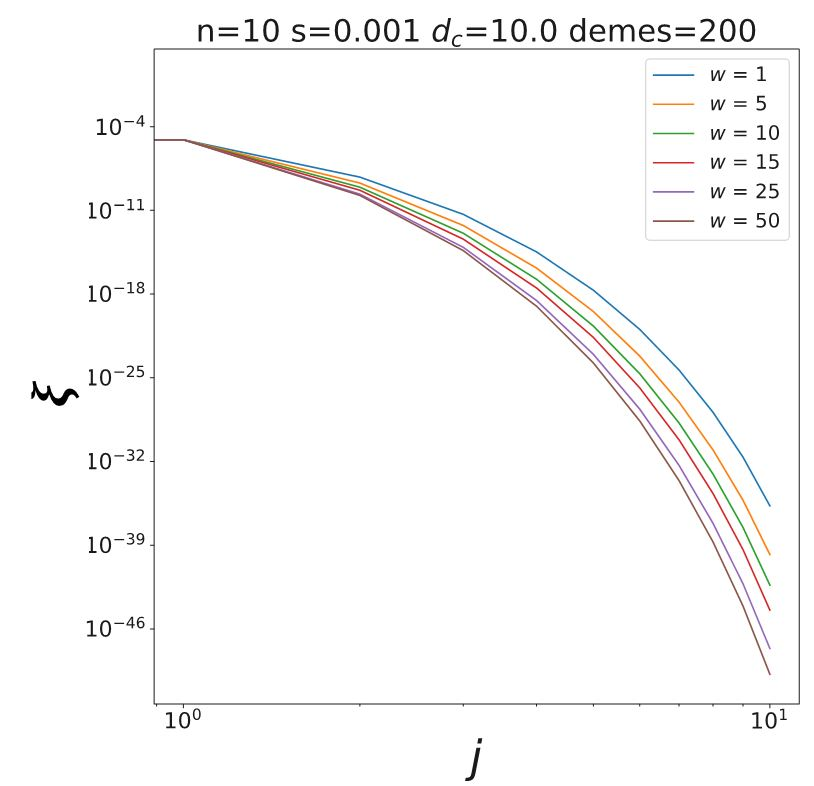
\includegraphics[scale=0.5]{img/sfs.JPG}
    \caption{The expected SFS $\xi$ decays as number of allele copies $j$ increases. As sampling width gets broader, the probability of detecting the same number of allele copies decays faster.}
    \label{fig:sfs}
\end{figure}


We describe the trade-off between narrow and broad sampling in figure \ref{fig:sampling_curves}. 

\begin{figure}[H]
    \centering
    \hspace*{-2cm}
    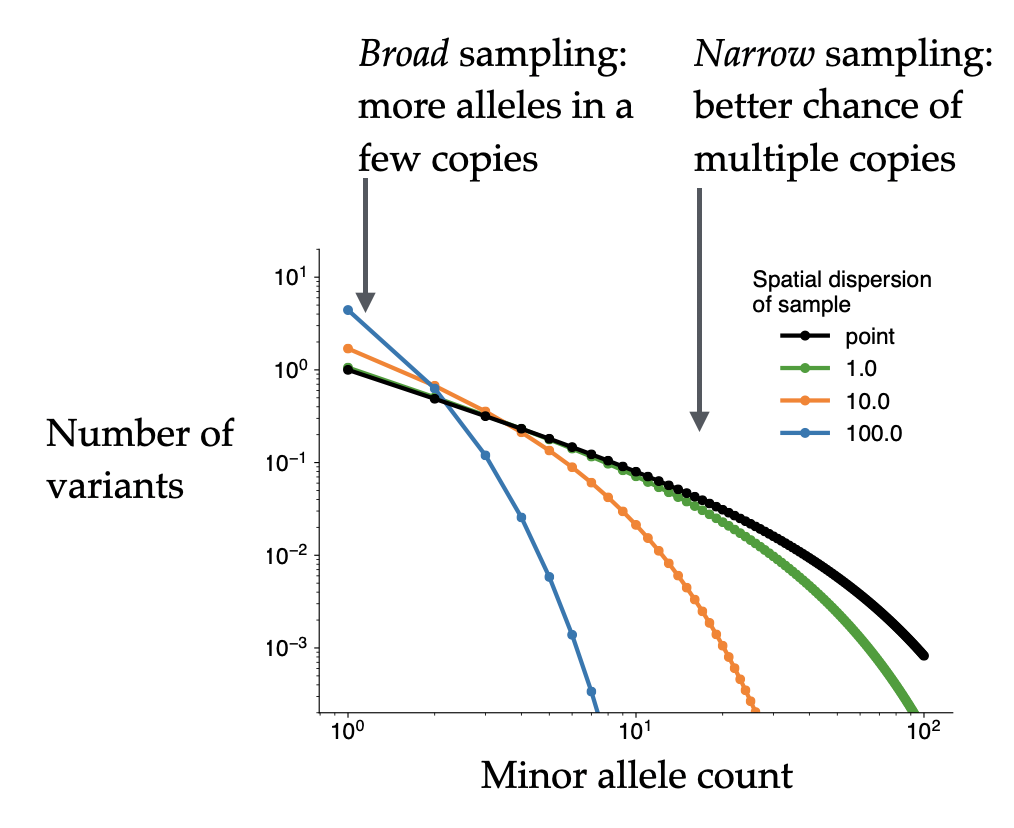
\includegraphics[scale=0.7]{img/sampling_curves.png}
    \caption{Each curve describes an increasing sample spatial dispersion $w$. The figure shows that broad sampling decreases the number of allele copies $j$ in  each sample, but detects alleles from a greater number of sites (more diverse population sample). Narrow sampling produces a less diverse sample (fewer sites detected), but improves the chance of observing multiple copies of alleles at each site.}
    \label{fig:sampling_curves}
\end{figure}




\newpage
\section{Measuring Missing Heritability}

In the final section of our results, we describe an application of our theoretical framework to tackle the problem of missing heritability. Upon entering the era of large-scale genomic data collection, researchers were optimistic that the recent plethora of information could effectively be used to explain the genetic basis of complex traits. Genome-wide association studies promised to identify genetic variants associated with disease. While many have provided insight into the genetic architecture of some diseases, most GWAS-identified variants explain little of the total variation in phenotype. \cite{manolio_finding_2009} The remaining, unexplained variation in phenotype has been dubbed "missing heritability" and many studies have recently attempted to solve the problem of missing heritability. \cite{young_solving_2019} 


One possible explanation for the missing heritability problem is that rare variants contribute much more strongly to disease risk than previously thought \cite{saint_pierre_how_2014} \cite{marouli_rare_2017}. Rare variants are more difficult to detect in GWAS, hence they are missing from the set of associated variants for a particular trait. Using our model, we compute the fraction of heritability explained in a "perfect GWAS" where every allele is detectable and contributes to the variance in the trait. 

Total heritability $H^2_T$ is traditionally written as the fraction of variance in phenotype $P$ that is explained by the variance in genotype $G$:


\begin{equation}
    H^2_T = \frac{Var[G]}{Var[P]}
\end{equation}


We compute the fraction of heritability explained by sampling from our spatial simulation. We define $H^2(w)$ as the ratio of the observed heritability $H^2_O$ to the total heritability $H^2_T$ as a function of sampling width $w$:

\begin{equation}
    \begin{split}
        H^2(w) &= \frac{H^2_O}{H^2_T} \\
        &= \frac{Var[G]_O}{Var[G]_T} \\ 
        &= \frac{\sum_{k=1}^{K} f_k(1-f_k) \textbf{P}}{\sum_{k=1}^{K} f_k(1-f_k)}
    \end{split}
\end{equation}

Where:
\begin{itemize}
    \item $\textbf{P}$ is a matrix which contains the probability of sampling the allele at each deme. It is computed from the sampled distribution of allele frequencies $\textbf{F}$ according to equation \ref{eq:psamp}.
    \item $K$ represents the number of independent replicate simulations performed for each set of population parameters
    \item $w$ is the standard deviation of the Gaussian sampling kernel
    \item $f_k$ is the allele frequency at a focal deme selected to be some distance from the center of the sampling kernel. As we move further away from the center of the distribution, we are increasing the distance between the focal deme and the center of the sampling kernel.
\end{itemize}

We compute matrix $\textbf{P}$ as the probability of observing all possible number combinations of $j$ allele copies in a sample of size $n$, ignoring the cases where $j = 0$ (no alleles in sample) and $j = n$ (entire sample contains copies of the allele). This calculation is similar to the expected SFS calculation \ref{eq:sfs}. 

\begin{equation}\label{eq:psamp}
    \begin{split}
    \textbf{P} &= \sum_{j=1}^{n-1} {n \choose j} F^j (1-F)^{n-j} \\
    &= 1 - {n \choose 0}F^0(1-F)^n - {n \choose n}F^n (1-F)^0 \\
    &= 1- (1-F)^n - F^n
    \end{split}
\end{equation}


\begin{figure}[H]
    \centering
    \hspace*{-1.5cm}
    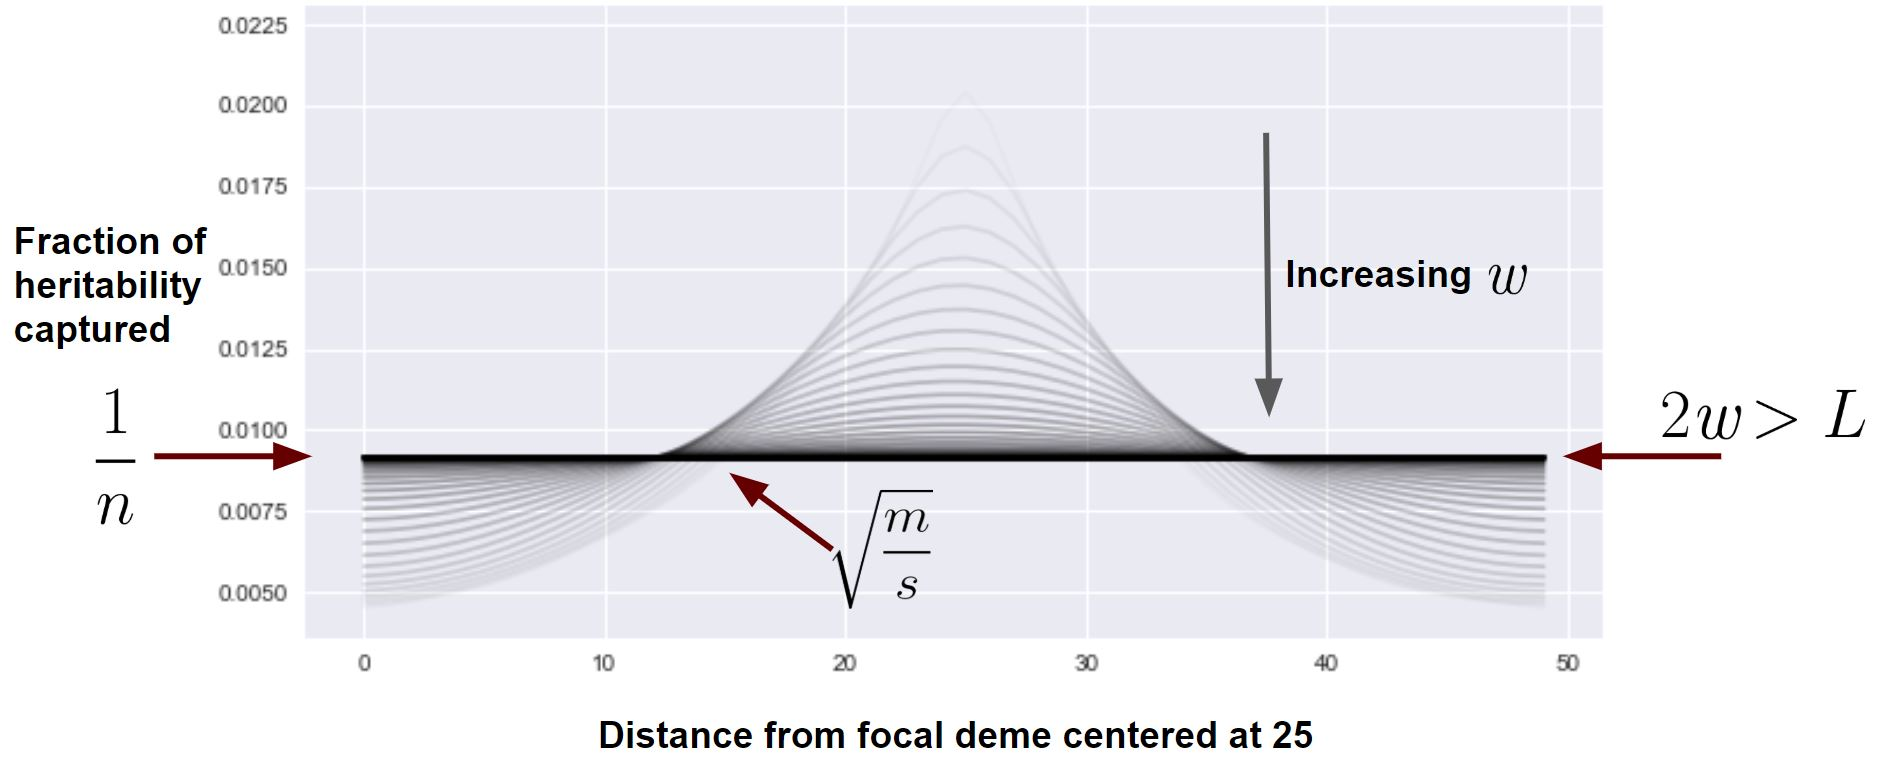
\includegraphics[scale=0.4]{img/heritability.JPG}
    \caption{$\bf{H^2}$ decreases as distance from the sampling center increases. We observe a trade-off between narrow and broad sampling. $\bf{H^2}$ is maximized when distance from focal deme $k =0$ and sampling is narrow.}
    \label{fig:missing_h}
\end{figure}

This result demonstrates the utility of our model. We have described the influence of spatial structure, selection, and sampling strategy on the observed distribution of allele frequencies. We have presented a trade-off between sampling many people from a broad geographic range (entire continent) or sampling the same number of people from a narrower range (country). If a particular GWAS aims to identify as many associated variants as possible, broader sampling is recommended. Still, this limits the maximum heritability explained to $\frac{1}{N}$. However, if a GWAS aims to capture as much heritability as possible or improve the chance of obtaining enough copies of an allele to detect a strong association, narrower sampling is recommended.


Further work on the relationship between our population parameters and $H^2$ is to be done. Ultimately, this model aims to provide a framework for relating the core evolutionary forces to the statistical trends observed in our analysis. We hope to apply our predictions to real population data, and contribute to the scientific conversation on improving the utility of GWAS.


%%%%% extra
